\documentclass{exam}
\date{28 Giugno 2017}
\usepackage[italian]{babel}
\usepackage[T1]{fontenc}
\usepackage{graphicx}
\title{Misura dell'accelerazione di gravit\'a}
\author{Francesco Sacco}
\usepackage{amsmath}
\usepackage{mathtools}
\usepackage{booktabs}


\begin{document}
	\maketitle
	\section{Scopo dell'esperienza}
		Lo scopo dell'esperienza \'e misurare l'accelerazione di gravit\'a

	\section{Apparato Sperimentale}
		\begin{itemize}
			\item Molla
			\item Piattello
			\item Supporto per la molla
			\item Pesetti da 50g,20g, due da 10g e uno da 5g
			\item Metro a nastro
			\item Cronometro
		\end{itemize}
	\section{Cenni Teorici}
		Il periodo $T$ di una molla di massa non trascurabile \'e uguale a 
		\begin{equation}
			T=2\pi \sqrt{\frac{m_p+m_i+m_m/3}{k}} 
		\end{equation}
		dove $m_p$ \'e la massa del piattello, $m_i$ \'e la somma delle masse poggiate sul piattello, $m_m$ \'e la massa della molla e $k$ \'e la costante di allungamento della molla.\newline
		Essendo tutti di dati noti, eccetto per $k$ \'e possibile usare questa equazione per ricavarsi la costante di allungamento.\newline\newline
		In condizione di riposo la molla si allunga secondo la seguente equazione		
		\begin{equation}
			\Delta l=\frac{(m_p+m_i)g}{k}
		\end{equation}
		dove $\Delta l$ \'e l'allungamento e $g$ \'e l'accelerazione di gravit\'a.\newpage
	\section{Raccolta dati}
		Il primo set di misure \'e stato effettuato per determinare il peso delle masse $m_i$ e l'allungamento della molla.
		\begin{center}
			\begin{tabular}{ll}
				\toprule
				$m_i(g)$&$\Delta l(cm)$\\
				\midrule
				$19,998\pm0,001$&$7,6\pm0,05$\\
				$30,001\pm0,001$&$11,4\pm0,05$\\
				$39,970\pm0,001$&$15,0\pm0,05$\\
				$50,017\pm0,001$&$18,6\pm0,05$\\
				\bottomrule
			\end{tabular}
		\end{center}
		Il Secondo set di Misurazioni \'e sto effettuato per vedere come varia il periodo $T$ in 10 oscillazioni al variare della massa $m_i$, nella seguente tabella ho messo i periodi gi\'a processati dal file python.
		\begin{center}
			\begin{tabular}{ll}
				\toprule
				$m_i(g)$&$T(s)$\\
				\midrule
				$19,998\pm0,001$&$0,703\pm0,021$\\
				$30,001\pm0,001$&$0,784\pm0,002$\\
				$39,970\pm0,001$&$0,871\pm0,001$\\
				$50,017\pm0,001$&$0,953\pm0,001$\\
				\bottomrule
			\end{tabular}
		\end{center}
	\section{Analisi dati}
		%Smorzato -------------------------------------------------------------------------
		\subsection{Misura di $k$}
			Dopo aver calcolato il periodo medio e la deviazione standard ho effettuato un fit con le masse lungo l'asse delle x e i periodi al quadrato sull'asse delle y, cos\'i facendo \'e possibile determinare $k$ con un fit lineare\\

			\begin{minipage}{0.5\textwidth}
				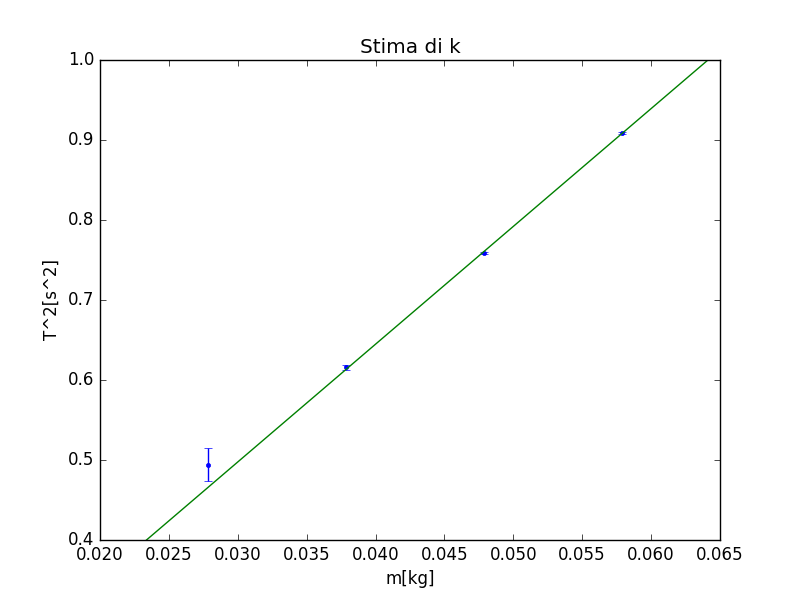
\includegraphics[width=\textwidth]{fit_k}
				\end{minipage}
			\begin{minipage}{0.5\textwidth}
				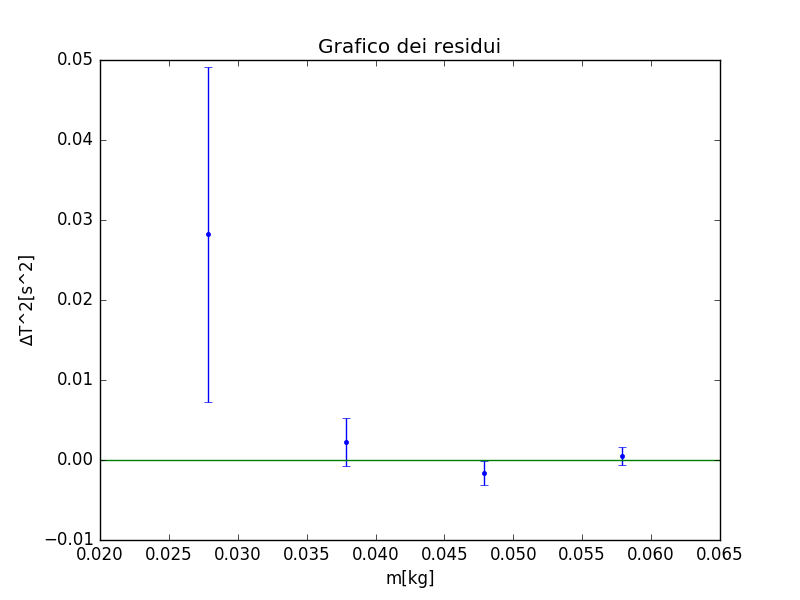
\includegraphics[width=\textwidth]{red_k}
			\end{minipage}
			\begin{center}
				\begin{tabular}{ll}
					\toprule
					Dati \\
					\midrule
					$k=2,681$ n/m $\pm0.001$ n/m\\
					$\chi^2=1,487$\\
					pValue=$0.171$\\
					dof=$4$\\		
					\bottomrule
				\end{tabular}
			\end{center}
		\subsection{Misura di $g/k$}
			In seguito ho effettuato le misure dell'allungamento della molla e fatto un fit lineare dove il coefficente angolare \'e $g/k$\\
			\begin{minipage}{0.5\textwidth}
					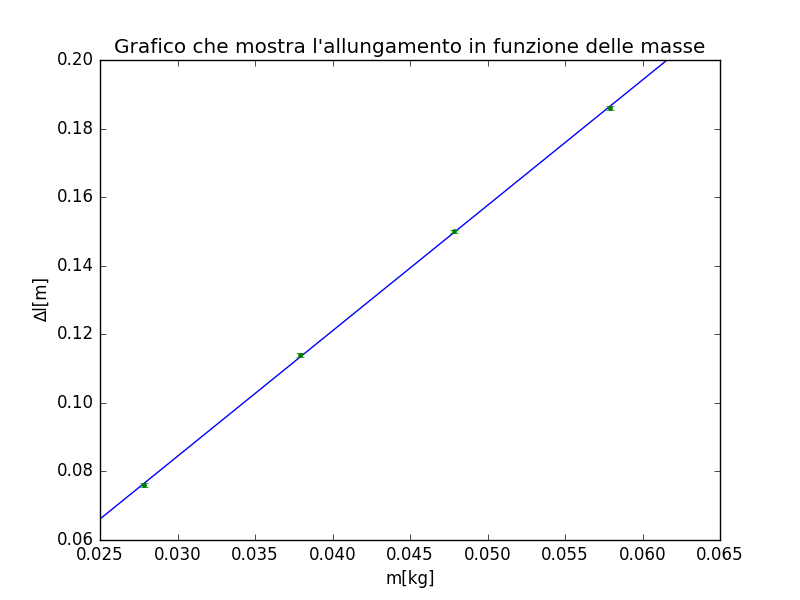
\includegraphics[width=\textwidth]{fit_kg}
			\end{minipage}
			\begin{minipage}{0.5\textwidth}
					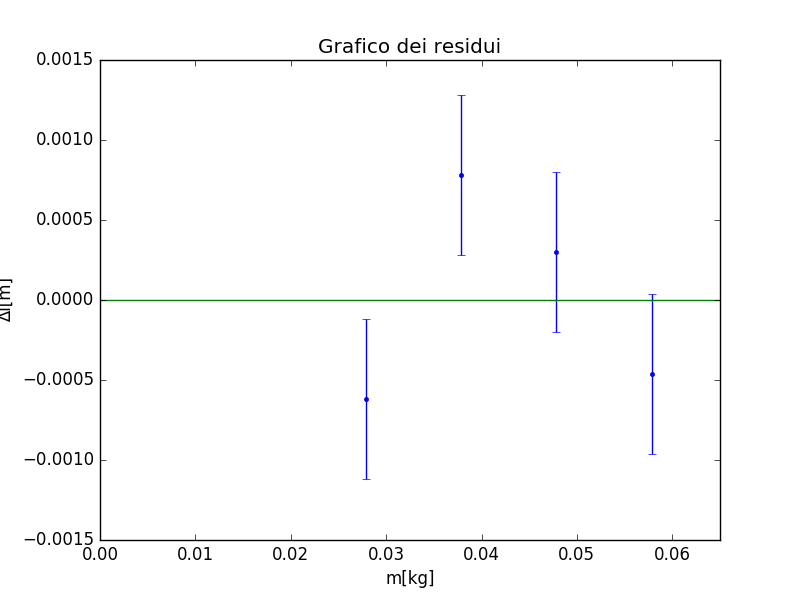
\includegraphics[width=\textwidth]{red_kg}
			\end{minipage}
				\begin{center}
				\begin{tabular}{ll}
						\toprule
						Dati \\
						\midrule
						$k/g=3,659$ kg m $\pm0.001$ kg m\\
						$\chi^2=5,175$\\
						pValue=$0.730$\\
						dof=$4$\\		
						\bottomrule	
					\end{tabular}
				\end{center}
		\subsection{Calcolo di g}
			Conoscendo $k$ e $g/k$ moltiplicando le medie e propagando l'errore sul prodotto si ottiene che $g=9,811\pm 0.007$.

	\section{Conclusione}
		Con i dati raccolti e la loro elaborazione \'e stato possibile ottenere una buona approssimazione dell'accelerazione di gravit\'a.

\end{document}